% #####################################################################
% #####################################################################
% ##                                                                 ##
% ##                             Lizenz:                             ##
% ##                         CC BY-NC-SA 3.0                         ##
% ##      http://creativecommons.org/licenses/by-nc-sa/3.0/de/       ##
% ##                                                                 ##
% #####################################################################
% ##   Diese Datei kann beliebig verändert werden, solange darauf    ##
% ##     hingewiesen wird, dass dieses Dokument ursprünglich von     ##
% ##                                                                 ##
% ##                        www.ei-studium.de                        ##
% ##                                                                 ##
% ##                             stammt.                             ##
% ## Dies gilt insbesondere auch für alle daraus erstellten Dateien. ##
% ##    Des Weiteren muss die Weitergabe dieser Dateien unter der    ##
% ##                    gleichen Lizenz erfolgen.                    ##
% #####################################################################
% #####################################################################
\documentclass[a4paper,twocolumn,10pt]{article}
\usepackage[utf8]{inputenc}
\usepackage[ngerman]{babel}
\usepackage[top=2.0cm,bottom=1.5cm,left=1.0cm,right=1.0cm]{geometry}
\usepackage{enumitem}
\usepackage{graphicx}
\usepackage{amsfonts}
\usepackage{amsmath}
\usepackage{sectsty}
\usepackage{colortbl}
\usepackage{cancel}
\usepackage{listings}
\usepackage{color}
\usepackage{amsmath}
\usepackage{trfsigns}
\usepackage{epstopdf}
\usepackage{amssymb}
\usepackage{fancyhdr}
\usepackage[pdfborder={0 0 0}]{hyperref}

\setlist{itemsep=.01mm}
\setenumerate{label=\emph{\arabic*})}
\setlength{\columnsep}{1cm}
\parindent 0mm

\partfont{\Large}
\sectionfont{\large \sc\bf}
\subsectionfont{\normalsize}
\subsubsectionfont{\small\textit}

\pagestyle{fancy}
\lhead[\leftmark]{Formelsammlung Technische Mechanik für EI}
\chead[\leftmark]{\url{http://www.ei-studium.de}}
\rhead[\leftmark]{Erstelldatum: \today}
\lfoot[\leftmark]{Keine Garantie auf Vollständigkeit und Richtigkeit!}
\cfoot[\leftmark]{}
\rfoot[\leftmark]{\thepage}
\renewcommand{\headrulewidth}{0.5pt}
\renewcommand{\footrulewidth}{0.5pt}

\begin{document}
\tableofcontents
\cleardoublepage

\part{Technische Mechanik}

\section{Stereo-Statik}

\subsection{Kräftesystem}

\subsubsection{Moment}

\begin{equation*}
\underline{M}^P=\underline{r}_{PO}\times\underline{F}
\end{equation*}

\subsubsection{Kraftwinder}
Der Kraftwinder stellt die Repräsentation aller an einen Körper angreifenden Kräfte durch ein äquivalentes Paar aus einer Kraft $\underline{F}$ und einem Moment $\underline{M}^P$ im Punkt $P$ dar:
\begin{equation*}
\begin{split}
(\underline{F}_1,\underline{F}_2,...,\underline{F}_n)&\sim (\underline{F},\underline{M}^P)\\
\underline{F}&=\sum\limits_{i}\underline{F}_i\\
\underline{M}^P&=\sum\limits_{i}(\underline{r}_{PP_{i}}\times \underline{F}_i)
\end{split}
\end{equation*}

\subsubsection{Statische Gleichgewichtsbedingungen}
\begin{equation*}
\begin{split}
(\underline{F},\underline{M}^P)&=(0,0)\\
\sum\limits_{i}\underline{F}_i&=0\\
\sum\underline{M}^P=\sum\limits_{i}(\underline{r}_{PP_i}\times\underline{F}_i)+\sum\limits_{j}\underline{M}_j&=0
\end{split}
\end{equation*}

\subsection{Ebene Statik}

\subsubsection{Freiheitsgrad}
Der Freiheitsgrad $g$ eines ungebundenen Körpers stellt die Anzahl der unabhängigen Bewegungsmöglichkeiten dar.
\begin{enumerate}
\item In der Ebene gilt: $g=3$
\item Im Raum gilt: $g=6$
\end{enumerate}

\subsubsection{Wertigkeit}
Die Wertigkeit $w$ ist die Anzahl der Freiheitsgrade, die eine Bindung (Gelenk, Lager) einschränkt.\\
Da Bindungen die Bewegungsmöglichkeiten eines Systems reduzieren, müssen sie dem System Kräfte in der eingeschränkten Bewegungsrichtung entgegensetzen. Diese Kräfte heißen \textbf{Reaktionen}. Es gilt:
\begin{equation*}
w_n=(s-1)\cdot h
\end{equation*}
mit $s$: Anzahl der beteiligten Stäbe und $h=2$ in der Ebene.
\begin{enumerate}[label=$\bullet$]
\item Loslager: $w=1$
\item Festlager: $w=2$
\item Feste Einspannung: $w=3$
\item Gelenk: $w=2$ für 2 Körper
\item Parallelführung: $w=2$
\end{enumerate}
\begin{center}
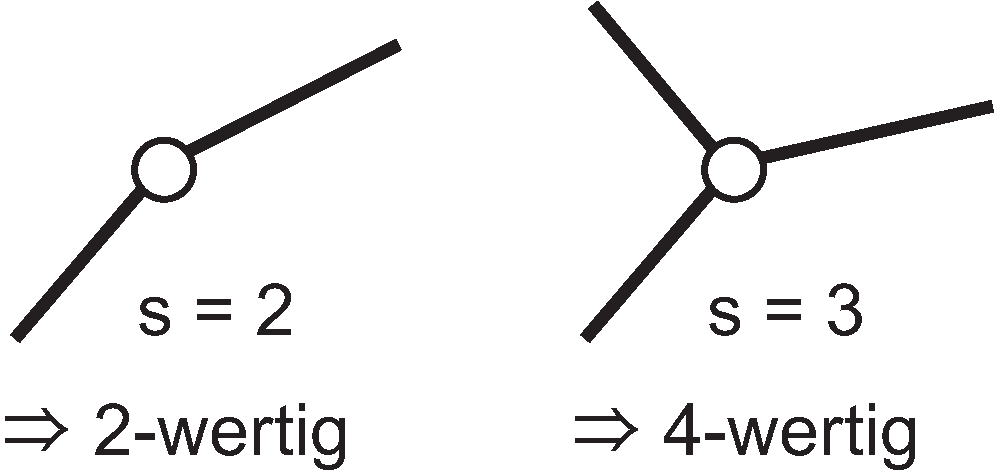
\includegraphics[width=0.6\columnwidth]{Grafiken/Bindungen_Wertigkeit}
\end{center}

\subsubsection{Statische und kinematische Bestimmtheit}
Eine Lagerung heißt:
\begin{enumerate}[label=$\bullet$]
\item \textbf{kinematisch bestimmt}, wenn sie die Lage eines Körpers eindeutig festlegt\\ ($\rightarrow$ keine Bewegungsmöglichkeiten)
\item \textbf{kinematisch unbestimmt}, wenn sich ein Körper um seine Ruhelage bewegen kann (endlich oder infinitesimal)
\item \textbf{statisch bestimmt}, wenn die Lagerreaktionen eindeutig aus dem GGW bestimmt werden können
\item \textbf{statisch unbestimmt}, wenn das GGW nicht ausreicht, um die Lagerreaktionen zu bestimmen (''statisch überbestimmt'')
\end{enumerate}
Notwendige Bedingung für die statische und kinematische Bestimmtheit:
\begin{equation*}
f=\underbrace{g\cdot i}_{\text{''Anzahl Gleichungen''}}-\underbrace{\sum\limits_{n=1}^{j}w_n}_{\text{''Anzahl Unbekannte''}}
\end{equation*}
$g$: Freiheitsgrade eines Körpers\\
$i$: Anzahl der Körper\\
$j$: Anzahl der Lager\\
$w_n$: Wertigkeit der $n$-ten Bindung\\\\
Es gilt:
\begin{enumerate}[label=$\bullet$]
\item $f=0$:\\
Notwendige (aber nicht hinreichende) Bedingung für statische und kinematische Bestimmtheit
\item $f<0$:\\
System $|f|$-fach statisch unbestimmt (überbestimmt)\\
$\rightarrow$ Elastostatik
\item $f>0$:\\
System $|f|$-fach kinematisch unbestimmt (unterbestimmt)\\
$\rightarrow$ Kinematik/Kinetik
\end{enumerate}

\subsection{Schwerpunkt}
Der Bezugspunkt $S$, der bei beliebiger Orientierung eines Körpers in einem parallelen Gravitationsfeld den Kraftwinder $(\underline{F},\underline{M})=(\underline{G},\underline{0})$ ergibt, heißt Schwerpunkt des Körpers:
\begin{equation*}
\begin{split}
\underline{G}&=\sum\limits_i\Delta\underline{G}_i=\sum\limits_i\Delta G_i\underline{e}\\
\underline{M}^S&=\sum\limits_i (\underline{r}_{SP_i}\times\Delta\underline{G}_i)=\sum\limits_i (\underline{r}_{SP_i}\Delta G_i)\times \underline{e}=\underline{0}
\end{split}
\end{equation*}
wobei $\underline{e}$ den normierten Vektor in Richtung der Erdbeschleunigung darstellt.

\subsubsection{Ort des Schwerpunktes}
Der Ort des Schwerpunktes errechnet sich wie folgt:
\begin{equation*}
\underline{r}_{OS}=\frac{1}{m}\int\limits_m\underline{r}_{OP}dm
\end{equation*}
Sonderfälle bei konstanter Dichte\\
(Volumendichte, Flächendichte, Liniendichte):
\begin{equation*}
\begin{split}
\underline{r}_{OS} &=\frac{1}{V}\int\limits_K \underline{r}_{OP}dV\\
\underline{r}_{OS}&= \frac{1}{A}\int\limits_K\underline{r}_{OP}dA\\
\underline{r}_{OS}&=\frac{1}{L}\int\limits_K\underline{r}_{OP}dL
\end{split}
\end{equation*}
Der Schwerpunkt liegt immer auf Symmetrieebenen/-achsen (falls vorhanden).
\begin{center}
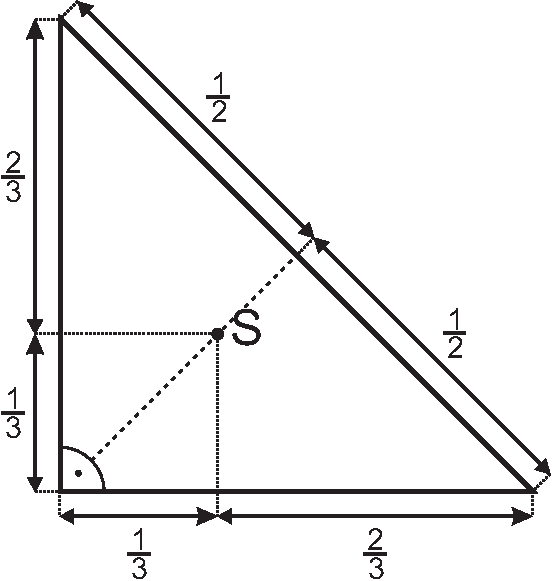
\includegraphics[width=0.5\columnwidth]{Grafiken/Schwerpunkt_Dreieck}
\end{center}

\subsubsection{Schwerpunkt bei mehreren Teilkörpern}
Bei Körpern, die sich aus mehreren Teilkörpern zusammensetzen, gilt für den Gesamtschwerpunkt:
\begin{equation*}
\begin{split}
\underline{r}_{OS}&=\frac{\sum\limits_i m_i\underline{r}_{OS_i}}{\sum m_i}\\\\
\underline{r}_{OS}&=\frac{\sum\limits_i V_i\underline{r}_{OS_i}}{\sum V_i}\\\\
\underline{r}_{OS}&=\frac{\sum\limits_i A_i\underline{r}_{OS_i}}{\sum A_i}
\end{split}
\end{equation*}

\subsection{Innere Kräfte und Momente am Balken}

\subsubsection{Schnittgrößen}
Schnittgrößen sind die inneren Lasten am Balken, die äußere Lasten aufnehmen und weiterleiten.\\\\
Vorzeichenkonvention:\\
Positive Schnittgrößen zeigen am positiven Schnittufer in positive Koordinatenrichtung:
\begin{center}
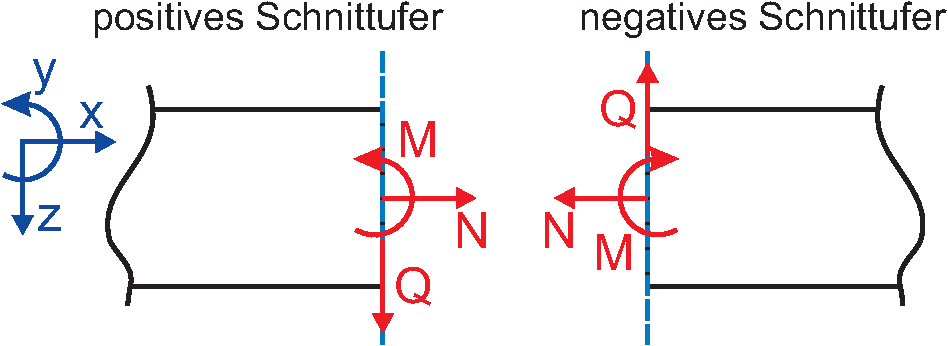
\includegraphics[width=0.65\columnwidth]{Grafiken/Schnittufer}
\end{center}
\begin{tabular}{ll}
$N$: & Normalkraft\\
$Q$: & Querkraft\\
$M$: & Biegemoment\\
$q$: & Streckenlast
\end{tabular}

\subsubsection{Föppl-Notation}
Es gilt:
\begin{equation*}
\langle x-a\rangle^n=\begin{cases}0 & \text{falls }x-a<0 \\ (x-a)^n & \text{falls }x-a>0\end{cases}
\end{equation*}

\subsubsection{Zusammenhänge}
\begin{equation*}
\begin{split}
q(x)&=-\frac{dQ(x)}{dx}\\
Q(x)&=-\int\limits_{0}^xq(\xi)d\xi -\sum F_i\langle x-x_i\rangle^0\\
Q(x)&=\frac{dM(x)}{dx}\\
M(x)&=\int\limits_0^x Q(\xi)d\xi -\sum M_j\langle x-x_j\rangle^0\\
N(x)&=-\sum F_k\langle x-x_k\rangle^0
\end{split}
\end{equation*}
\begin{tabular}{ll}
$F_i$: & Kräfte in positive $z$-Richtung\\
$F_k$: & Kräfte in positive $x$-Richtung\\
$M_j$: & Momente in positiver Drehrichtung
\end{tabular}

\subsubsection{Allgemeine Vorgehensweise}
\begin{enumerate}
\item Bestimmung der Lagerreaktionen
\begin{enumerate}
\item Freischnitt des Balkens an Lagerstellen
\item Ersetzen von Streckenlasten durch ihre Resultierenden im Kraftangriffspunkt
\item Bestimmung der Lagerreaktionen aus den GGW-Bedingungen
\end{enumerate}
\item Bestimmung der Schnittreaktionen
\begin{enumerate}
\item Freischnitt des betrachteten Balkens von allen Lagern und Anbauten
\item Aufstellen der Funktion der Streckenlast $q(x)$
\item Berechnung von $Q(x)$ und $M(x)$ mit Integrationsformeln
\end{enumerate}
\item Alternative Bestimmung der Schnittreaktionen
\begin{enumerate}
\item Freischnitt des betrachteten Balkens von allen Lagern und Anbauten
\item Freischneiden eines Teils des betrachteten Balken und Einzeichnen der Schnittreaktionen $N(x),Q(x)$ und $M(x)$.
\item Berechnung der Schnittreaktionen durch Aufstellen von GGW-Bedingungen
\end{enumerate}
\end{enumerate}

\subsection{Reibung}

\subsubsection{Gleitreibung}
\begin{equation*}
|F_R|=\mu\cdot F_N
\end{equation*}
$\mu$: Gleitreibkoeffizient

\subsubsection{Haftreibung}
\begin{equation*}
|F_R|\leq \mu_0\cdot F_N
\end{equation*}
$\mu_0$: Haftreibkoeffizient

\section{Elastostatik}

\subsection{Spannung}
\begin{center}
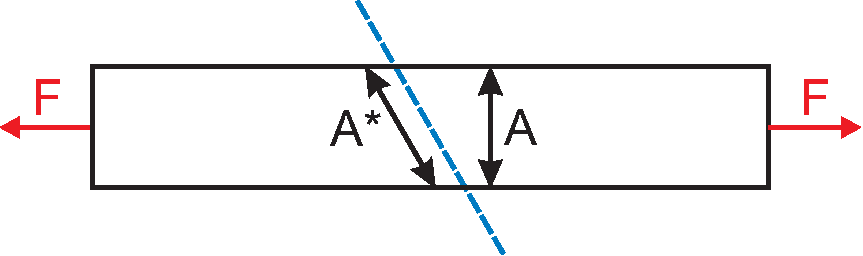
\includegraphics[width=0.65\columnwidth]{Grafiken/Stab_Spannung}
\end{center}
\begin{tabular}{ll}
$\sigma$: & Normalspannung (normal zu $A^*$)\\
$\tau$: & Schubspannung (tangential zu $A^*$)
\end{tabular}
\begin{equation*}
\begin{split}
\sigma&=\frac{F_N}{A^*}=\frac{F_Ncos(\varphi)}{A};\;\;\;\;F_N=F\cdot cos(\varphi)\\
\tau&=\frac{F_T}{A^*}=\frac{F_Tcos(\varphi)}{A};\;\;\;\;F_T=F\cdot sin(\varphi)
\end{split}
\end{equation*}
Für die maximalen Spannungen gilt:
\begin{equation*}
\begin{split}
\sigma_{\text{max}}&=\sigma(\varphi=0)=\frac{F}{A}\\
\tau_{\text{max}}&=\tau\left(\varphi=\frac{\pi}{4}\right)=\frac{1}{2}\frac{F}{A}
\end{split}
\end{equation*}
Dimensionierung eines Stabes:
\begin{equation*}
\begin{split}
|\sigma_{\text{max}}|&\leq\sigma_{\text{zul}}\\
A_{\text{min}}&\geq\frac{|F|}{\sigma_{\text{zul}}}
\end{split}
\end{equation*}

\subsection{Dehnung}
\begin{tabular}{ll}
$\epsilon$: & Dehnung\\
$u$: & Längenänderung
\end{tabular}
\begin{equation*}
\begin{split}
\epsilon&=\frac{\Delta l}{l}\;\;\;\;\text{falls }\epsilon\text{ konstant}\\
\epsilon(x)&=\frac{du(x)}{dx}\\
u(x)&=\int\epsilon(x)dx
\end{split}
\end{equation*}

\subsection{Stoffgesetz}
\begin{equation*}
\begin{split}
\sigma&=E\cdot\epsilon\\
\epsilon_T&=\alpha_T\Delta T\\
\epsilon&=\epsilon_M+\epsilon_T=\frac{\sigma}{E}+\alpha_T\Delta T\\
\frac{du}{dx}&=\frac{N}{EA}+\alpha_T\Delta T\\
\Delta l&=u(l)-u(0)=\int\limits_0^l\epsilon(x)dx
\end{split}
\end{equation*}
Falls $\Delta T=0;N=F=const.; EA=const.$:
\begin{equation*}
\Delta l=\frac{Fl}{EA}
\end{equation*}
\begin{tabular}{ll}
$\epsilon_T$: & Thermische Dehnung\\
$\alpha_T$: & Thermischer Ausdehnungskoeffizient\\
$u(x)$: & Verschiebung\\
$E$: & Elastizitätsmodul
\end{tabular}

\subsection{Allgemeine Vorgehensweise}
\begin{enumerate}
\item Bei statisch bestimmten Problemen
\begin{enumerate}
\item Bestimmung der Normalkraft aus GGW am Teilsystem/-element
\item Berechnung der Spannung aus der Belastung und Berechnung der Dehnung aus dem Stoffgesetz
\item Bestimmung der Verschiebung bzw. Längenänderung durch Integration
\end{enumerate}
Temperaturänderung führt nur zu thermischer Dehnung
\item Bei statisch unbestimmten Problemen
\begin{enumerate}
\item Normalkraft kann nicht aus GGW am Teilsystem/-element bestimmt werden
\item GGW, geometrische Verträglichkeit und Elastizitätsgesetz müssen gleichzeitig betrachtet werden.
\end{enumerate}
Temperaturänderung kann zu zusätzlicher Spannung führen
\end{enumerate}

\section{Kinematik}

\subsection{Starrkörperkinematik}
\begin{equation*}
\begin{split}
\underline{v}_i&=\underline{\omega}\times\underline{r}_i\\
\omega&=\frac{d\varphi}{dt}\\
\underline{v}_Q&=\underline{v}_P+\underline{\omega}\times\underline{r}_{PQ}\;\;\;\;\text{Starrkörperformel}
\end{split}
\end{equation*}

\subsubsection{Momentanpol im ebenen Fall}
Die allgemeine Bewegung eines Starrkörpers kann immer als eine Drehung um einen Punkt, den Momentanpol $MP$ beschrieben werden.

\subsubsection{Allgemeine Vorgehensweise}
\begin{enumerate}
\item Fixe $MP$ suchen
\begin{enumerate}[label=$\rightarrow$]
\item Festlager
\item Abrollendes Rad auf Umgebung
\end{enumerate}
\item Fixe Geschwindigkeiten suchen
\begin{enumerate}[label=$\rightarrow$]
\item Loslager
\item Gleiten
\item Polstrahlen verlaufen senkrecht zur Geschwindigkeit
\end{enumerate}
\item Schnittpunkt von Polstrahlen zweier körperfester Punkte = $MP$
\item Gelenke/Gemeinsame Punkte zweier Körper
\begin{enumerate}[label=$\rightarrow$]
\item Gleiche Geschwindigkeiten
\end{enumerate}
\item Die Polstrahlen aller Punkte auf einem Stab verlaufen durch einen gemeinsamen $MP$
\end{enumerate}

\subsection{Relativkinematik}

\subsubsection{Koordinatentransformation}
Es gilt:
\begin{equation*}
\begin{split}
{}_I\underline{r}_{PA}&= {}_I\underline{e}_x^K {}_Kx^*+ {}_I\underline{e}_y^K {}_Ky^*+ {}_I\underline{e}_z^K {}_Kz^*;\;\;\;\;{_K}\underline{r}_{PA}=\begin{pmatrix}{}_Kx^* \\ {}_Ky^* \\ {}_Kz^*\end{pmatrix}\\
{}_I\underline{r}_{PA}&=\underbrace{\left({}_I\underline{e}_x^K,{}_I\underline{e}_y^K,{}_I\underline{e}_z^K\right)}_{A_{IK}}\begin{pmatrix}{}_Kx^* \\ {}_Ky^* \\ {}_Kz^*\end{pmatrix}\\
{}_I\underline{r}_{PA}&=A_{IK}\cdot{}_K\underline{r}_{PA}
\end{split}
\end{equation*}
${}_I\underline{e}_i^K$ ist hierbei der $i$-te Einheitsvektor des $K$-Systems, dargestellt im $I$-System.\\\\
Für die Transformationsmatrix gilt:
\begin{equation*}
\begin{split}
A_{KI}&=A_{IK}^{-1}\\
A_{KI}&=A_{IK}^T\;\;\;\;\text{falls }A_{IK}\text{ orthogonal}\\
A_{31}&=A_{32}A_{21}
\end{split}
\end{equation*}

\subsubsection{Elementardrehungen}
\begin{equation*}
\begin{split}
A_x(\alpha)&=\begin{pmatrix}1 & 0 & 0 \\ 0 & cos(\alpha) & sin(\alpha) \\ 0 & -sin(\alpha) & cos(\alpha)\end{pmatrix}\;\;\;\;\text{Drehung um }x\text{-Achse}\\
A_y(\beta)&=\begin{pmatrix}cos(\beta) & 0 & -sin(\beta) \\ 0 & 1 & 0 \\ sin(\beta) & 0 & cos(\beta)\end{pmatrix}\;\;\;\;\text{Drehung um }y\text{-Achse}\\
A_z(\gamma)&=\begin{pmatrix}cos(\gamma) & sin(\gamma) & 0 \\ -sin(\gamma) & cos(\gamma) & 0 \\ 0 & 0 & 1\end{pmatrix}\;\;\;\;\text{Drehung um }z\text{-Achse}
\end{split}
\end{equation*}

\subsubsection{Zeitableitung}
Ist ein Vektor $a$ in einem drehenden $KOSY$ $K$ gegeben, muss bei der Zeitableitung die Produktregel beachtet werden:
\begin{equation*}
\begin{split}
{}_K\underline{a}&=\sum a_i\underline{e}_i^K\\
\Rightarrow {}_K\underline{\dot{a}}&=\sum \dot{a}_i\underline{e}_i^K+\sum a_i\underline{\dot{e}}_i^K
\end{split}
\end{equation*}
Alternativ kann die Euler'sche Differentiationsregel angewendet werden.

\subsubsection{Euler'sche Differentiationsregel}
Der Eulerterm muss immer dann berücksichtigt werden, wenn die absolute zeitliche Ableitung eines Vektors in einem bewegten $KOSY$ dargestellt werden soll:
\begin{equation*}
{}_K\underline{\dot{a}}={}_K\underline{\overset{\circ}{a}}+{}_K\underline{\omega}_K\times {}_K\underline{a}
\end{equation*}

\subsubsection{Allgemeine Vorgehensweise}
\begin{enumerate}
\item Zweckmäßige $KOSY$ (körperfest) einführen
\item Transformationsmatrizen bestimmen
\item Ortsvektoren im passenden System aufstellen\\
$\rightarrow$ möglichst einfache Beschreibung wählen
\item Winkelgeschwindigkeitsvektor drehender Systeme aufstellen
\item Geschwindigkeiten durch Differentiation bestimmen\\
$\rightarrow$ Eulerterm bei bewegten Systemen
\item Beschleunigungen durch Differentiation bestimmen\\
$\rightarrow$ Eulerterm bei bewegten Systemen
\end{enumerate}

\section{Kinetik}

\subsection{Grundbegriffe}
Impuls $dp$ eines Masseelements $dm$:
\begin{equation*}
d\underline{p}=\underline{v}_pdm=\frac{d\underline{r}_p}{dt}dm
\end{equation*}
Impuls $p$ eines Körpers:
\begin{equation*}
\underline{p}=\int\limits_Kd\underline{p}=\int\limits_K\underline{v}_pdm
\end{equation*}
Impuls $p$ eines Körpers mit konstanter Masse $m$:
\begin{equation*}
\underline{p}=m\underline{v}_S
\end{equation*}

\subsection{Impuls}
Impulssatz eines Masseteilchens $dm$:
\begin{equation*}
\frac{d}{dt}\underline{p}=\frac{d}{dt}(\underline{v}dm)=d\underline{F}
\end{equation*}
Impulssatz eines Körpers:
\begin{equation*}
\frac{d}{dt}\underline{p}=\underline{F}
\end{equation*}
Impulssatz eines Körpers mit konstanter Masse:
\begin{equation*}
m\underline{a}_S=\underline{F}
\end{equation*}

\subsubsection{Sonderfälle}
\textbf{Impulserhaltungssatz:}
\begin{equation*}
\underline{F}=\underline{0}\Rightarrow \underline{\dot{p}}=0\Rightarrow\underline{p}=const.
\end{equation*}
\textbf{Statik:}
\begin{equation*}
\underline{a}_S=\underline{0}\Rightarrow\underline{F}=\underline{0}
\end{equation*}

\subsection{Drall und Massenträgheit}

\subsubsection{Drall}
Drall eines Masseelements mit Geschwindigkeit $\underline{v}_P$ bzgl. eines ruhenden Punktes $O$:
\begin{equation*}
d\underline{L}^{O}=\underline{r}_{OP}\times d\underline{p}=\underline{r}_{OP}\times(\underline{v}_Pdm)
\end{equation*}
Drall eines Körpers bzgl. eines ruhenden Punktes $O$:
\begin{equation*}
\underline{L}^{O}=\int\limits_Kd\underline{L}^{O}=\int\limits_K(\underline{r}_{OP}\times\underline{v}_P)dm
\end{equation*}
Wechsel des Bezugspunktes, ausgehend vom Schwerpunkt
\begin{enumerate}[label=$\bullet$]
\item auf beliebigen Punkt $Q$:
\begin{equation*}
\underline{L}^Q=\underline{L}^S+m(\underline{r}_{QS}\times\underline{v}_{QS})
\end{equation*}
\item auf Fixpunkt $O$:
\begin{equation*}
\underline{L}^{O}=\underline{L}^S+\underline{r}_{OS}\times \underline{p}
\end{equation*}
\end{enumerate}

\subsubsection{Drallsatz}
Drallsatz eines Starrkörpers bzgl. beliebigem Punkt $Q$:
\begin{equation*}
\underline{M}^Q=\frac{d}{dt}\underline{L}^Q+m(\underline{r}_{QS}\times\underline{a}_Q)
\end{equation*}
Drallsatz eines Starrkörpers bzgl. ruhendem Punkt $O$ bzw. Schwerpunkt $S$:
\begin{equation*}
\underline{M}^{O}=\underline{\dot{L}}^{O};\;\;\;\;\underline{M}^S=\underline{\dot{L}}^S
\end{equation*}

\subsubsection{Massenträgheit}
\begin{equation*}
{}_K\underline{L}^S=\underbrace{\begin{pmatrix}\Theta_{xx} & -\Theta_{xy} & -\Theta_{xz} \\ -\Theta_{yx} & \Theta_{yy} & -\Theta_{yz} \\ -\Theta_{zx} & -\Theta_{zy} & \Theta_{zz}\end{pmatrix}}_{{}_K\Theta^S}\underbrace{\begin{pmatrix}\omega_x \\ \omega_y \\ \omega_z\end{pmatrix}}_{{}_K\underline{\omega}}
\end{equation*}
Der Massenträgheitstensor ${}_K\Theta^S$ ist symmetrisch.
\begin{equation*}
\begin{split}
\Theta_{xx}&=\int\limits_Ky^2+z^2dm\\
\Theta_{yy}&=\int\limits_Kx^2+z^2dm\\
\Theta_{zz}&=\int\limits_Kx^2+y^2dm\\
\Theta_{xy}&=\Theta_{yx}=\int\limits_Kxydm\\
\Theta_{xz}&=\Theta_{zx}=\int\limits_Kxzdm\\
\Theta_{yz}&=\Theta_{zy}=\int\limits_Kyzdm
\end{split}
\end{equation*}

Änderung des Bezugssystems:
\begin{equation*}
{}_H\Theta^S=A_{HK}\cdot {}_K\Theta^S\cdot A_{HK}^T
\end{equation*}

\subsubsection{Sonderfälle}
\begin{enumerate}
\item Drehung um feste Achse durch $S$:\\
Beispiel: Drehung um $z$-Achse
\begin{equation*}
{}_K\underline{\omega}=\begin{pmatrix}0 \\ 0 \\ \omega\end{pmatrix}\Rightarrow {}_K\underline{L}^S=\begin{pmatrix}-\Theta_{xz} \\ -\Theta_{yz} \\ \Theta_{zz}\end{pmatrix}\cdot\omega
\end{equation*}
\item Drehung um feste Achse durch $S$ mit symmetrischer Massenverteilung um Rotationsachse:\\
Beispiel: Drehung um $z$-Achse
\begin{equation*}
\Theta_{xz}=\Theta_{yz}=0;\;{}_K\underline{\omega}=\begin{pmatrix}0 \\ 0 \\ \omega\end{pmatrix}\Rightarrow {}_K\underline{L}^S=\begin{pmatrix}0 \\ 0 \\ \Theta_{zz}\end{pmatrix}\cdot\omega
\end{equation*}
\end{enumerate}

\subsubsection{Satz von Steiner}
Für die Verschiebung des Koordinatenursprungs gilt:
\begin{equation*}
\begin{split}
{}_K\underline{r}_{SB}&=\begin{pmatrix}a \\ b \\ c\end{pmatrix}
\end{split}
\end{equation*}
\begin{equation*}
\begin{split}
&{}_K\Theta^B=\\
&\begin{pmatrix}\Theta_{xx}+(b^2+c^2)m & -(\Theta_{yx}+abm) & -(\Theta_{xz}+acm) \\ -(\Theta_{xy}+abm) & \Theta_{yy}+(a^2+c^2)m & -(\Theta_{yz}+bcm) \\ -(\Theta_{zx}+acm) & -(\Theta_{zy}+bcm) & \Theta_{zz}+(a^2+b^2)m\end{pmatrix}
\end{split}
\end{equation*}

\subsubsection{Allgemeine Vorgehensweise}
\begin{enumerate}
\item Einführung geeigneter Koordinatensysteme
\item Freischnitt aller Körper und Eintrag aller Schnittreaktionen
\item Aufstellen der absoluten (Winkel-)Beschleunigung aller Körper (Relativkinematik)
\item Bestimmung der Trägheitsmomente/-tensoren der Körper
\item Aufstellen von Impuls- und Drallsätzen
\item Kopplung über Kinematik und Schnittreaktionen
\end{enumerate}
\textbf{Tipp:}\\
Der Impulssatz lässt sich meist leichter im Inertialsystem, der Drallsatz im körperfesten System (konst. Trägheitstensor) auswerten!

\subsection{Energie}

\subsubsection{Kinetische Energie}
Kinetische Energie $dT$ eines Masseelements $dm$:
\begin{equation*}
dT=\frac{1}{2}\underline{v}^T\underline{v}dm=\frac{1}{2}v^2dm
\end{equation*}
Kinetische Energie $T$ eines Starrkörpers:
\begin{equation*}
T=\int\limits_KdT=\frac{1}{2}\int\limits_Kv^2dm=\frac{1}{2}\int\limits_Kv^Tdp
\end{equation*}
Mit Hilfe der Starrkörperkinematik gilt:
\begin{equation*}
T=\underbrace{\frac{1}{2}m\underline{v}_Q^2}_{\text{translat.}}+\underbrace{m\underline{v}_Q^T(\underline{\omega}\times\underline{r}_{QS})}_{\text{Koppelterm}}+\underbrace{\frac{1}{2}\underline{\omega}^T\underline{L}^Q}_{\text{rotat.}}
\end{equation*}

\subsubsection{Sonderfälle}
\begin{enumerate}
\item Bezugspunkt $Q$ = Schwerpunkt $S$:
\begin{equation*}
T=\frac{1}{2}m\underline{v}_S^2+\frac{1}{2}\underline{\omega}^T\Theta^S\underline{\omega}
\end{equation*}
\item Bezugspunkt $Q$ = Momentanpol $M$:
\begin{equation*}
T=\frac{1}{2}\underline{\omega}^T\Theta^M\underline{\omega}
\end{equation*}
\end{enumerate}

\subsubsection{Konservative Kräfte und potentielle Energie}
\textbf{Definitionen:}
\begin{enumerate}[label=$\bullet$]
\item Ist die Arbeit einer Kraft zur Verschiebung eines Massenteilchens unabhängig von der Bahnkurve, heißt die Kraft \textbf{konservativ}.
\item Die \textbf{potentielle Energie} $V$ ist ein Maß für die Fähigkeit einer konservativen Kraft $F$ Arbeit $W$ zu leisten.
\end{enumerate}

\subsubsection{Energiesatz}
In einem konservativen Kraftfeld ist die Summe aus kinetischer und potentieller Energie konstant:
\begin{equation*}
T+V=E=const.
\end{equation*}

\subsubsection{Allgemeine Vorgehensweise}
\begin{enumerate}
\item Wahl eines geeigneten Bezugsniveaus für die potentielle Energie
\item Bestimmung der kinetischen und potentiellen Energien in den Punkten $(1)$ und $(2)$ aller Körper
\item Bei nichtkonservativen Systemen:\\
Bestimmung der Arbeit zwischen den Punkten $(1)$ und $(2)$
\item Aufstellen der Energiebilanz/-erhaltung zwischen den Punkten $(1)$ und $(2)$
\end{enumerate}

\cleardoublepage

\section{Verständnisfragen}

\subsection{Stereo-Statik}

\subsubsection{Kräftesystem}
\textbf{Durch welche Eigenschaften ist eine Kraft definiert?}\\
Durch Betrag, Richtung und Angriffspunkt.\\\\
\textbf{Unter welcher Voraussetzung kann eine Kraft als ein linienflüchtiger Vektor betrachtet werden?}\\
Wenn der Körper starr ist, d.h. wenn der Körper unter Einfluss von Kräften keine Deformation erfährt.\\\\
\textbf{Was besagt das Schnittprinzip?}\\
Zum ''Sichtbarmachen'' von Schnitt- und Reaktionskräften wird das System als starr angenommen und an den Systemgrenzen freigeschnitten.\\
Ist das Gesamtsystem im GGW, sind auch Teilsysteme im GGW.\\
Alle Kräfte außerhalb des Schnittes werden hierdurch zu äußeren Kräften.\\\\
\textbf{Was sind äußere Kräfte?}\\
Kräfte, die von außen auf den Körper einwirkten.\\\\
\textbf{Was ist eine Reaktionskraft?}\\
Reaktionskräfte bzw. Lagerkräfte sind Kräfte, die den eingeprägten Kräften entgegengerichtet sind, sodass der Körper im GGW bleibt.\\\\
\textbf{Wie kann ein Moment mit Kräften ausgedrückt werden?}\\
Ein Moment $M$ kann durch eine Kraft $F$ ausgedrückt werden, die an einem Hebelarm angreift:
\begin{equation*}
\underline{M}^P=\underline{r}_{PO}\times \underline{F}
\end{equation*}
\textbf{Was ist ein Kraftwinder?}\\
Ein Kraftwinder stellt die Repräsentation aller an einen Körper angreifenden Kräfte durch ein äquivalentes Paar aus einer Kraft $\underline{F}$ und einem Moment $\underline{M}^P$ im Punkt $P$ dar.\\\\
\textbf{Welche Komponente eines Kraftwinders ändert sich bei einem Wechsel des Bezugspunktes?}\\
Das Moment ändert sich.

\subsubsection{Ebene Statik}
\textbf{Welchen Bedingungen muss ein Kräftesystem genügen, wenn es im GGW sein soll?}\\
Die Summe aller Kräfte und Momente muss Null ergeben.\\\\
\textbf{Wie viele GGW-Bedingungen können für einen Körper in der Ebene aufgestellt werden?}\\
Es können drei GGW-Bedingungen aufgestellt werden.\\\\
\textbf{Welche GGW-Bedingungen können für eine ebenes, zentrales Kräftesystem aufgestellt werden?}\\
Es können zwei GGW-Bedingungen aufgestellt werden (Kräfte in x- und y-Richtung). Das Momenten-GGW liefert keine weitere Aussage.\\\\
\textbf{Worin unterscheiden sich die Bauelemente Seil, Stab und Balken?}\\
Ein Seil überträgt nur Zugkräfte, ein Stab überträgt Zug- und Druckkräfte und ein Balken kann sowohl beliebige Kräfte als auch Momente übertragen.\\\\
\textbf{Wie ist der Begriff Lagerwertigkeit definiert?}\\
Anzahl der Freiheitsgrade, die ein Lager einschränkt.\\\\
\textbf{Wie groß ist die Lagerwertigkeit eines Drehgelenks, das drei Körper in der Ebene verbindet?}\\
Das Lager ist 4-wertig.\\\\
\textbf{Wie groß ist die Zahl der Lagerreaktionen in einem räumlichen Kugelgelenk?}\\
{\color{red}keine Ahnung.}\\\\
\textbf{Wann ist ein Körper kinematisch bestimmt gelagert?}\\
Wenn die Lage des Körpers eindeutig festgelegt ist (keine Bewegungsmöglichkeiten).\\\\
\textbf{Wann ist ein Körper 3-fach statisch unbestimmt gelagert?}\\
Wenn es im zugehörigen Gleichungssystem drei Gleichungen mehr als Unbekannte gibt.

\subsubsection{Schwerpunkt}
\textbf{Welche Richtung hat die Gewichtskraft?}\\
Die Gewichtskraft zeigt nach unten (in Richtung des Erdmittelpunktes).\\\\
\textbf{Wie ist der Schwerpunkt eines Körpers definiert?}\\
Der Bezugspunkt $S$, der bei beliebiger Orientierung eines Körpers in einem parallelen Gravitationsfeld den Kraftwinder $(\underline{F},\underline{M})=(\underline{G},\underline{0})$ ergibt.\\\\
\textbf{Wann fällt der Schwerpunkt mit dem Volumenmittelpunkt eines Körpers zusammen?}\\
Wenn der Körper eine konstante Dichte besitzt.\\\\
\textbf{Wie viele Symmetrieebenen eines homogenen Körpers sind nötig, um den Schwerpunkt ohne weitere Rechnung zu bestimmen?}\\
Die Anzahl der notwendigen Symmetrieebenen entspricht der Anzahl der Dimensionen des Raumes.

\subsubsection{Innere Kräfte und Momente}
\textbf{Wie sind die inneren Kräfte Normalkraft $N$, Querkraft $Q$ und Biegemoment $M$ bei einem Balken definiert?}\\
Das sind die inneren Lasten am Balken, die äußere Lasten aufnehmen und weiterleiten:\\\\
\begin{tabular}{ll}
Normalkraft $N$: & Normal zur Schnittfläche\\
Querkraft $Q$: & In der Schnittebene\\
Biegemoment $M$: & Resultierendes Moment bzgl. des\\
& Schwerpunktes der Schnittfläche.
\end{tabular}\\\\\\
\textbf{Welche Beziehungen gelten zwischen $q(x),Q(x)$ und $M(x)$ bei einem Balken?}\\
\begin{equation*}
q(x)=-\frac{dQ(x)}{dx};\;\;\;\;Q(x)=\frac{dM(x)}{dx}
\end{equation*}\\
\textbf{Wie ist das positive Schnittufer definiert?}\\
\begin{center}
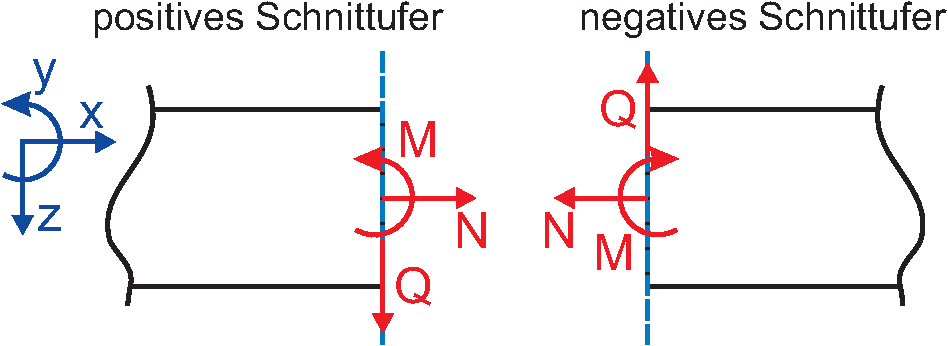
\includegraphics[width=0.65\columnwidth]{Grafiken/Schnittufer}
\end{center}
\textbf{Welchen Einfluss haben diskrete Kräfte auf $N(x),Q(x)$ und $M(x)$?}\\
Diskrete Kräfte verursachen einen Sprung in $N(x)$ und $Q(x)$ bzw. einen Knick in $M(x)$.\\\\
\textbf{In welchen Fällen wird eine Streckenlast durch die Resultierende ersetzt?}\\
Zur Bestimmung der Lagerreaktionen.\\\\
\textbf{Wie wird eine bei $x=a$ in $z$-Richtung angreifende Einzelkraft in $Q(x)$ mit Hilfe von Föppl-Klammern berücksichtigt?}\\
\begin{equation*}
Q(x)=-F\cdot\langle x-a\rangle^0
\end{equation*}

\subsubsection{Reibung}
\textbf{Welche Kräfte treten in einem Reibkontakt auf?}\\
Normalkraft $F_N$ und Reibkraft $F_R$.\\\\
\textbf{Welche Zustände unterscheidet das Reibgesetz nach Coulomb?}\\
Haften und Gleiten.\\\\
\textbf{Wie wird die Haft- und wie die Gleitreibkraft bestimmt?}\\
Die Haftreibkraft ist eine Reaktionskraft und wird aus den GGW-Bedingungen bestimmt.\\
Die Gleitreibkraft ist eine eingeprägte Kraft und wirkt entgegen der Bewegungsrichtung. Sie wird bestimmt durch: $|F_R|=\mu\cdot F_N$\\\\
\textbf{Ist die Haftreibkraft eine eingeprägte oder eine Reaktionskraft?}\\
Eine Reaktionskraft.\\\\
\textbf{Wie ist der Reibkegel definiert?}\\
Ein Körper bleibt in Ruhe (haftet), so lange die resultierende Kraft $F_{\text{res}}$ aus Normalkraft $F_N$ und Reibkraft $F_R$ innerhalb des Reibkegels liegt ($\mu_0=tan(\varphi_0)$).

\subsection{Elastostatik}
\textbf{Welche Spannungskomponenten treten in einem allgemeinen Schnitt durch einen Stab auf?}\\
Normalspannungen und Schubspannungen.\\\\
\textbf{Welche Kenngrößen sind wichtig bei der Dimensionierung eines Stabes?}\\
Die maximale Normalspannung $\sigma_{\text{max}}$.\\\\
\textbf{Unter welcher Voraussetzung stimmen globale und lokale Dehnung überein?}\\
Wenn die lokale Dehnung konstant ist, d.h. wenn der Stab an jeder Stelle gleichmäßig erwärmt wird, einen konstanten Temperaturkoeffizienten, die gleiche Querschnittsfläche und die gleiche Normalkraft hat.\\\\
\textbf{Was ist der Unterschied zwischen Längung, Dehnung, Stauchung und Verschiebung?}\\
Dehnung ist die lokale Längenänderung, Längung ist die Längenänderung des Stabes.\\\\
\textbf{Welche Dehnungskomponenten kennen Sie?}\\
Mechanische und thermische Dehnung.\\\\
\textbf{Welche Bereiche finden sich in einem Spannungs-Dehnung-Diagramm?}\\
Linear-elastischer Bereich, Fließbereich, Verfestigungsbereich und Einschnürungsbereich.\\\\
\textbf{Wie lautet das Hookesche Stoffgesetz?}\\
$\sigma=E\cdot \epsilon$\\\\
\textbf{Wann führt eine thermische Spannung zu einer mechanischen Belastung eines Stabsystems?}\\
Wenn das System statisch unbestimmt ist.

\subsection{Kinematik}

\subsubsection{Starrkörperkinematik}
\textbf{Wie werden Teildrehgeschwindigkeiten mathematisch zusammengefasst?}\\
Teildrehgeschwindigkeiten werden addiert.\\\\
\textbf{Welche geometrische Beziehung besteht zwischen Geschwindigkeit und Polstrahl?}\\
Geschwindigkeit $\perp$ Polstrahl\\\\
\textbf{Wie ist der Momentanpol eines Körpers definiert?}\\
Die allgemeine Bewegung eines Starrkörpers kann immer als eine Drehung um einen Punkt, den Momentanpol $MP$ beschrieben werden.\\\\
\textbf{Wo befindet sich der Momentanpol eines translatorisch bewegten Körpers?}\\
Im Unendlichen.\\\\
\textbf{Wie kann aus der Winkelgeschwindigkeit und der Geschwindigkeit eines Punktes die Schwerpunktsgeschwindigkeit eines Starrkörpers bestimmt werden?}\\
$\underline{v}_S=\underline{v}_P+\underline{\omega}\times\underline{r}_{PS}$

\subsubsection{Relativkinematik}
\textbf{Wie bestimmt man eine Transformationsmatrix?}\\
Eine Transformationsmatrix setzt sich aus den Einheitsvektoren des alten Systems, dargestellt im neuen System, zusammen.\\\\
\textbf{Welche Beziehung in den Matrizen besteht zwischen Transformation und Rücktransformation?}\\
Für orthogonale Transformationen gilt:\\
$A_{KI}=A_{IK}^T=A_{IK}^{-1}$\\\\
\textbf{In welcher Reihenfolge müssen aufeinanderfolgende Transformationsmatrizen multipliziert werden?}\\
$A_{31}=A_{32}A_{21}$\\\\
\textbf{Was ist der Eulerterm und wann muss er benutzt werden?}\\
Der Eulerterm muss immer dann berücksichtigt werden, wenn die absolute zeitliche Ableitung eines Vektors in einem bewegten $KOSY$ dargestellt werden soll:\\
${}_K\underline{\dot{a}}={}_K\underline{\overset{\circ}{a}}+{}_K\underline{\omega}_K\times {}_K\underline{a}$\\\\
\textbf{Was ist der Unterschied zwischen Absolut- und Relativgeschwindigkeit?}\\
Die Absolutgeschwindigkeit ist die Geschwindigkeit bezüglich der inertialen Basis $I$; Geschwindigkeiten bzgl. körperfester Basen sind Relativgeschwindigkeiten.\\\\
\textbf{Aus welchen Termen setzt sich die Absolutbeschleunigung in einem drehenden $KOSY$ zusammen?}\\
Aus Translations-, Relativ-, Rotations-, Coriolis-, Führungs- und Zentripetalbeschleunigung.

\subsection{Kinetik}

\subsubsection{Impuls}
\textbf{Wie ist der Impuls eines Starrkörpers definiert?}\\
$\underline{p}=\int\limits_K\underline{v}_pdm$\\\\
\textbf{Welcher geometrische Zusammenhang besteht zwischen Impuls und Schwerpunktsgeschwindigkeit?}\\
$\underline{p}=m\cdot\underline{v}_S$ falls Masse konstant.\\\\
\textbf{Wie lautet der Impulssatz für einen Starrkörper?}\\
$\frac{d\underline{p}}{dt}=\underline{F}$\\\\
\textbf{Wie lässt sich aus dem Impulssatz das Kräftegleichgewicht der Statik ableiten?}\\
Ist die Beschleunigung eines Systems Null, ist die resultierende äußere Kraft einer Nullkraft äquivalent:\\
$\underline{a}_S=\underline{0}\Rightarrow\underline{F}=\underline{0}$

\subsubsection{Drall und Massenträgheit}
\textbf{Wie werden die Einträge des Trägheitstensors genannt?}\\
Hauptdiagonale: Massenträgheitsmomente (MTM)\\
Nebendiagonale: Massendeviationsmomente (MDM)\\\\
\textbf{Wie ist ein Hauptachsensystem definiert?}\\
Jeder starre Körper besitzt drei zueinander senkrecht stehende Achsen (Hauptachsen), für die die MTM extremal werden und die MDM verschwinden.\\\\
\textbf{Wie bestimmt man den Trägheitstensor bei}\\
\textbf{a) Verschiebung des Bezugspunkts eines Starrkörpers?}\\
Mit Hilfe des Satzes von Steiner.\\\\
\textbf{b) Verdrehung der Koordinatenachsen eines Starrkörpers?}\\
${}_H\Theta^S=A_{HK}\cdot {}_K\Theta^S\cdot A_{HK}^T$\\\\
\textbf{Wie kann der Drall mit Hilfe des Trägheitstensors definiert werden?}\\
${}_K\underline{L}^S={}_K\Theta^S {}_K\underline{\omega}$\\\\
\textbf{Wann sind Drall- und Winkelgeschwindigkeitsvektor parallel?}\\
Bei einer Drehung um eine feste Achse mit symmetrischer Massenverteilung um die Rotationsachse.\\\\
\textbf{Wie lautet der Drallsatz bzgl. Körperschwerpunkt?}\\
$\underline{M}^S=\underline{\dot{L}}^S$

\subsubsection{Energie}
\textbf{Aus welchen Anteilen setzt sich die kinetische Energie zusammen?}\\
Translatorischer Anteil, Koppelterm und Rotatorischer Anteil.\\\\
\textbf{Ist die kinetische Energie abhängig vom Bezugspunkt?}\\
Ja.\\\\
\textbf{Was ist eine konservative Kraft?}\\
Ist die Arbeit einer Kraft zur Verschiebung eines Massenteilchens unabhängig von der Bahnkurve, heißt die Kraft konservativ.\\\\
\textbf{Kann ein absoluter Wert der potentiellen Energie eindeutig bestimmt werden?}\\
Nein, da die potentielle Energie vom Bezugspunkt abhängt.\\\\
\textbf{Wie lautet der Arbeitssatz?}\\
Die von einer Kraft $F$ beim Beschleunigen einer Punktmasse $dm$ geleistete Arbeit $dW$ ist gleich der Änderung der kinetischen Energie $dT$.\\\\
\textbf{Nennen Sie Beispiele für konservative und nicht-konservative Kräfte!}\\\\
\begin{tabular}{ll}
Konservative Kräfte: & Gewichtskraft, Federkraft\\
Nichtkonservative Kräfte: &Geschwindigkeitsproportionaler\\
& Dämpfer
\end{tabular}
\\\\\\\\
Lizenz: CC BY-NC-SA 3.0\\
\url{http://creativecommons.org/licenses/by-nc-sa/3.0/de/}

\end{document}








